% \documentclass[usenames,dvipsnames,9pt,pdf,utf8,russian,aspectratio=169]{beamer}
% \usepackage{cmap}%Пакеты для русского языка
% \usepackage{diagbox}%Пакеты для русского языка
% \usepackage[T2A]{fontenc}
% \usepackage[utf8]{inputenc}
% \usepackage[russian]{babel}
% \usepackage{graphicx} %Пакет для вставки рисунков

% %AMS TEX значки и пр.
% \usepackage{amssymb}
% \usepackage{amsthm}
% \usepackage{amsfonts}
% %разные пакеты
% \usepackage{wrapfig}
% %Нужно включать, если используется "тема" (стиль оформления) по умолчанию
% %\usepackage{beamerthemesplit}
% \usepackage{array}
% \usepackage{url}
% \usepackage{breakurl}
% \usepackage{wrapfig}
% \usepackage{changepage}   % for the adjustwidth environment

% \usepackage{cutwin}
	
% \usepackage{amsmath}

 

% \usepackage{tikz}
% \usetikzlibrary{trees}


% %Привычный шрифт для математических формул
% \usefonttheme[onlymath]{serif}
% %Общий стиль ("тема") оформления слайдов
% %Можно выбрать любую тему в \localtexmf\tex\latex\beamer\themes\theme\
% %и её имя подставить в качестве аргумента в \usetheme
% %Требование: чёрные буквы на белом фоне
% %\usetheme{Frankfurt}
% %Более крупный шрифт для подзаголовков титульного листа
% %\setbeamerfont{institute}{size=\normalsize}
% %Задание команды (\bluetext) для выделения конкретным (синим) цветом
% %(используйте \alert для выделения цветом выбранной "темы")
% \setbeamercolor{bluetext_color}{fg=blue}
% \newcommand{\bluetext}[1]{{\usebeamercolor[fg]{bluetext_color}#1}}
% \mode<presentation>
% {
%   \usetheme{Boadilla}      % or try Darmstadt, Madrid, Warsaw, ...
%   \usecolortheme{seagull} % or try albatross, beaver, crane, ..

%   \usefonttheme{structurebold}  % or try serif, structurebold, ...
%   \setbeamertemplate{navigation symbols}{}
%   \setbeamertemplate{caption}[numbered]
% } 



% %%Если используется последовательное появление пунктов списков на слайде
% %%(не злоупотребляйте в слайдах для защиты дипломной работы), чтобы
% %%еще непоявившиеся пункты были все-таки немножко видны.
% \setbeamercovered{transparent}
% \setbeamertemplate{navigation symbols}{}
% %\setbeamertemplate
% %{footline}
% %{\quad\strut
% %\hfill\insertframenumber/\inserttotalframenumber\strut\quad}
% \setlength{\topsep}{0pt}%
% \DeclareMathOperator{\cov}{cov}
% \DeclareMathOperator{\pow}{pow}
% \DeclareMathOperator{\med}{med}
% \DeclareMathOperator{\mymode}{mode}
% \DeclareMathOperator{\rank}{rank}
% \DeclareMathOperator{\arctanh}{arctanh}
% \DeclareMathOperator{\diag}{diag}
% \DeclareMathOperator{\sign}{sign}
% \DeclareMathOperator*{\plim}{\mathop{plim}}
% \DeclareMathOperator{\prob}{\mathbf{P}\!}

% \DeclareGraphicsExtensions{.pdf,.png,.jpg,.eps}

% \renewcommand{\leq}{\leqslant}
% \renewcommand{\geq}{\geqslant}

% \def\argmin#1{ \mathop{\text{argmin}}\limits_{#1} }
% \def\argmax#1{ \mathop{\text{argmax}}\limits_{#1} }
% %TODO - уточнить 43

% \DeclareMathOperator{\FWER}{FWER}
% \DeclareMathOperator{\FDR}{FDR}
% \newtheorem{Th}{Теорема}
% \newtheorem{Def}{Определение}
% \title[ПСАД-12. Марковские модели]{Прикладной статистический анализ данных\\ Марковские модели}
% \author[Олег Бахтеев]{Олег Бахтеев\\psad@phystech.edu}
% \date{2022}

% \begin{document}


\documentclass[9pt,pdf,utf8,hyperref={unicode},aspectratio=169]{beamer}

%Привычный шрифт для математических формул
\usefonttheme[onlymath]{serif}
\mode<presentation>
{
    \usetheme{boxes}
    \beamertemplatenavigationsymbolsempty

    \setbeamercovered{transparent}
    \setbeamertemplate{navigation symbols}{}
    
    \setbeamertemplate{footline}[frame number]
    \setbeamertemplate{caption}[numbered]
    % \setbeamersize{text margin left=0.5em, text margin right=0.5em}
}

% Дополнительные библиотеки
\usepackage[T2A]{fontenc}
\usepackage[english, russian]{babel}
\usepackage[utf8]{inputenc}
\usepackage{amsmath,amssymb}
\usepackage{indentfirst}
\usepackage{changepage}
\usepackage{enumerate}
\usepackage{mathtools}
\usepackage{multicol}
\usepackage{multirow}
\usepackage{ragged2e}
\usepackage{multicol}
\usepackage{diagbox}
\usepackage{wrapfig}
\usepackage{comment}
\usepackage{subfig}
\usepackage{array}
\usepackage{color}
\usepackage{tikz}
\usepackage{url}
\usepackage{bm}

\usetikzlibrary{trees}

% Определение дополнительных функций
\DeclareMathOperator*{\plim}{\mathop{plim}}
\DeclareMathOperator{\prob}{\mathbf{P}\!}

\DeclareMathOperator{\arctanh}{arctanh}
\DeclareMathOperator{\mmode}{mode}
\DeclareMathOperator{\rank}{rank}
\DeclareMathOperator{\diag}{diag}
\DeclareMathOperator{\sign}{sign}
\DeclareMathOperator{\cov}{cov}
\DeclareMathOperator{\pow}{pow}
\DeclareMathOperator{\med}{med}

\def\argmin#1{ \mathop{\text{argmin}}\limits_{#1} }
\def\argmax#1{ \mathop{\text{argmax}}\limits_{#1} }

\newcommand{\tsum}{\mathop{\textstyle\sum}\limits}
\newcommand{\condprob}[2] {\mathbf{P}\!\left(#1\left|#2\right.\right)}

\renewcommand{\leq}{\leqslant}
\renewcommand{\geq}{\geqslant}

\DeclareMathOperator{\FWER}{FWER}
\DeclareMathOperator{\FDR}{FDR}
\newtheorem{Th}{Теорема}
\newtheorem{Def}{Определение}

% Основная часть

\title[Марковские модели]{Прикладной статистический анализ данных\\Марковские модели}
\author{Андрей Грабовой}
\date{}

\begin{document}
\tikzstyle{every node}=[draw=black,thick,anchor=west]
\tikzstyle{selected}=[draw=red,fill=red!30]
\tikzstyle{optional}=[dashed,fill=gray!50]

\begin{frame}
    \titlepage
\end{frame}


\section{Марковская цепь}

\begin{frame}{Марковская цепь}
Последовательность дискретных случайных величин $X_1, \dots, X_T$, принимающих некоторый набор значений $\{O_1, \dots, O_m\}$, называется простой однородной цепью Маркова, если
\[
    P(X_{t+1} = O_{t+1}| X_{t}=O_{t}, \dots, X_1 = O_1) = P(X_{t+1} = O_{t+1}| X_{t}=O_{t}),
\]
\[
    P(X_{t+1} = O_{t+1}| X_{t}=O_{t}) \text{    не зависит от номера шага }t.
\]

\vspace{1cm}
Марковская цепь задается: 
\begin{itemize}
\item множеством наблюдаемых состояний $\{O_1, \dots, O_m\}$;
\item начальными значениями вероятности состояний $P(X_1 = O_i) = P_i$;
\item вероятностью перехода между состояниями $ P(X_{t} = O_{i}| X_{t-1}=O_{j}) = P_{ij}$.
\end{itemize}
\end{frame}

\subsection{Примеры}
\begin{frame}{Пример: погода}
Задан набор из трех состояний:
\begin{enumerate}
\item $O_1$ = дождливая погода;
\item $O_2$ = пасмурная погода;
\item $O_3$ = солнечная погода.
\end{enumerate}
\begin{itemize}
\item Какова вероятность, что в следующие четыре дня погода будет меняться как ``солнце-солнце-дождь-дождь''?
\[
    P(O_3, O_3, O_1, O_1) = P_3P_{33}P_{31}P_{11}
\]
\item Какова вероятность, что ровно $N$ дней будет пасмурная погода?
\[
    P(X_2 = O_2,\dots,X_t = O_2, X_{N} \neq O_2|X_1=O_2) = P_{22}^{N-1}(1-P_{22}).
\]
\item Ожидаемая продолжительность постоянной пасмурной погоды:
\[
    \mathsf{E} = \sum_{t=1}^\infty t \cdot P(X_2 = O_2,\dots,X_t = O_2, X_{t+1} \neq O_2|X_1=O_2) = \frac{1}{1-P_{22}}.
\]
\end{itemize}
\end{frame}
\subsection{Языковая модель}
\begin{frame}{Языковая модель}
Примером марковской цепи выступает языковая $n$-грамм модель.

Под $n$-граммой понимается последовательность из $n$ подряд идущих слов.\\

\textbf{Пример:}\\
\textit{Шла Саша по шоссе} содержит три $2$-граммы:
\begin{enumerate}
\item Шла Саша;
\item Саша по;
\item По шоссе.
\end{enumerate}

\end{frame}
\begin{frame}{Языковая модель}
Языковая модель позволяет оценить вероятность появления предложения на основе марковской модели языка.\vspace{0.2cm}\\

Для удобства при построении языковой модели вводятся два специальных символа:
\textit{BOS (Begin Of Sentence)} и \textit{EOS (End Of Sentence)}. \\
\vspace{0.2cm}
\textbf{Пример} для $3$-граммной языковой модели:
\begin{align}
&p(w_1,\dots,w_n)=  p(SOS) \times \nonumber \\[18pt]
&\times p(w_1|SOS)p(w_2|w_1,SOS)p(w_3|w_2,w_1)\dots p(w_{n}|w_{n-1},w_{n-2}) \nonumber \\[18pt]
&\times p(EOS|w_{n},w_{n-1}).\nonumber  
\end{align}
\end{frame}

\begin{frame}{Языковая модель: измерение качества}
%https://web.stanford.edu/~jurafsky/slp3/3.pdf
Как оценить качество модели?\\
\textbf{Кросс-Энтропия.}\\
Оценка на основе заданной выборки $w_1,\dots,w_n$:
\[
        H = -\frac{1}{n} \log p(w_1,\dots,w_n).
\]

\textbf{Перплексия:}
\[
        PP = 2^{H} = p(w_1,\dots,w_n)^{-\frac{1}{n}}.
\]
\begin{itemize}
\item $PP = \infty \to$ марковская цепь не описывает выборку;
\item $PP = 1 \to$ марковская цепь идеально описывает выборку.
\end{itemize}
\end{frame}


\begin{frame}{Языковая модель: незнакомые слова}
В случае, если языковой модели встретится неизвестное слово, $p(w_1, \dots, w_n) = 0$.

\textbf{Варианты работы с незнакомыми словами:}
\begin{itemize}
\item Сглаживание Лапласа:
\[
    p(w_i) = \frac{c_i+1}{\sum_{j=1}^v c_j + v}, 
\]
где $c_i$ --- встречаемость слова $w_i$ в тексте, $v$ --- мощность словаря.
\item Интерполяция моделей разных порядков:
\[
    \hat{p}(w_n|w_{n-1},w_{n-2}) = \lambda_1 p(w_n|w_{n-1},w_{n-2}) + \lambda_2 p(w_n|w_{n-1}) + \lambda_3 p(w_n),
\]
\[
     \quad \sum_i \lambda_i = 1.
\]

\end{itemize}
\end{frame}


\subsection{Проверка гипотез}
\begin{frame}{Марковские модели, проверки гипотез}
\only<1>{
\textit{Проверка гипотезы о соответствии вектора вероятностей $p_{i1}, \dots, p_{im}$ перехода из состояния $i$ заданному:}
\begin{center}
\begin{tabular}{rl}
            выборка:                        & $X_1, \dots, X_T$ \\
            нулевая гипотеза:               & $H_0\colon p_{i1}, \dots, p_{im}=\mathbf{p}^0$ \\
            альтернатива:                   & $H_1\colon p_{i1}, \dots, p_{im}\neq \mathbf{p}^0$ \\
            статистика:                     & $n_i \sum_{j}\frac{({p}_{ij}-p^{0}_{ij})^2}{p^{0}_{ij}},$ \\
                                            & где $n_i$ --- встречаемость наблюдения $O_i$ \\
                                            &  в последовательности $X_1, \dots, X_{T-1}$\\
            нулевое распределение:          & $\chi^2_{m-1}$\\
		\end{tabular}
		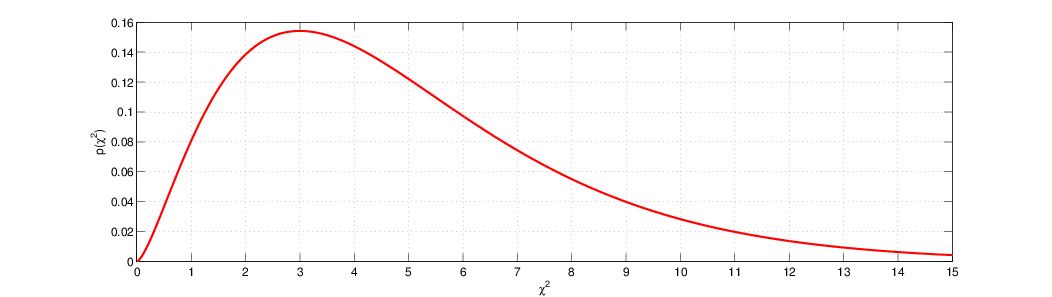
\includegraphics[width=0.85\textwidth]{chi2.png}   
    \end{center}
}
\only<2>{
\textit{Проверка гипотезы о том, что марковскую цепь второго порядка можно ``свернуть'' в цепь первого порядка:}
\begin{center}
\begin{tabular}{rl}
            выборка:                        & $X_1, \dots, X_T$, задана марковская модель порядка 2:\\
            ~                               & $P(X_t = O_k|X_{t-1} = O_{j}, X_{t-2} = O_{i}, \dots)= p_{ijk}$ \\
            нулевая гипотеза:               & $H_0\colon p_{1jk} = p_{2jk} =\dots = p_{mjk}.$ \\
            альтернатива:                   & $H_1\colon H_0$ неверна.  \\
            статистика:                     & $-2\text{log}\bigl(\prod_{i,j,k=1}^m(\hat{p}_{ij} / {p}_{ijk})^{n_{ijk}})\bigr),$ \\
            ~                               & $\hat{p}_{ij}$ --- оценка МП,\\
            ~                               & $n_{ijk}= |\{X_t: X_t = O_i, X_{t+1} = O_j, X_{t+2} = O_k\}|.$\\
            нулевое распределение:          & $\chi^2_{m(m-1)^2}$\\
		\end{tabular}
		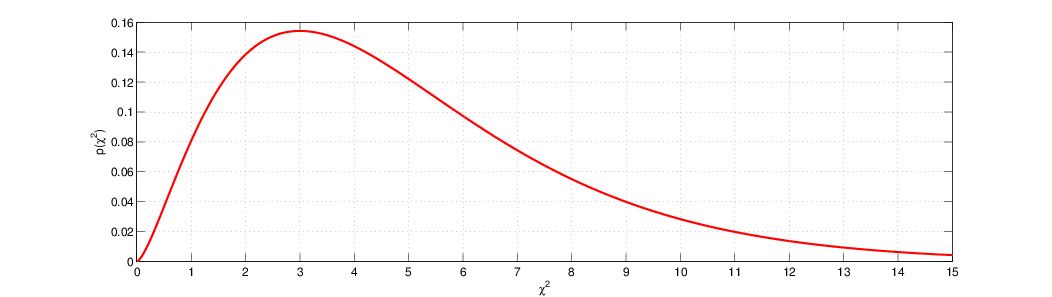
\includegraphics[width=0.85\textwidth]{chi2.png}   
    \end{center}
}
\end{frame}

\begin{frame}{Проверка гипотез, комментарии}
\begin{itemize}
\item Вероятностное распределение $p_{ij}$ представимо как мультиномиальное распределение события $j$ при условии события $i$, поэтому для проверки гипотез применимы критерии для мультиномиальных величин (в случае $m=2$ --- критерии для распределения Бернулли).
\item Предполагается, что все вероятности переходов при проверке гипотез строго больше нуля.
\item Критерии можно обобщить на случай моделей более высокого порядка (например, полагать $p_{ijk}$ моделью первого порядка с событием $X_t = O_k$ при условии \textit{единого} события $<X_{t-1} = O_{j}, X_{t-2} = O_i>$.
\item Возможна проверка критериев по нескольким последовательностям, а не по одной. Статистики и нулевая гипотеза от этого не меняются.
\item Подробнее --- см. Anderson et al. (в списке литературы).
\end{itemize} 
\end{frame}

\subsection{Порождающие модели}
\begin{frame}{Марковские модели как порождающие модели}
\textbf{Примеры порождающих моделей:}
\begin{itemize}
\item Генераторы поведения ветра (используются для изучения климата).
\item Генераторы текста (см. https://hackernoon.com/automated-text-generator-using-markov-chain-de999a41e047)\\        
\item SciGen: генератор псевдонаучных текстов
\begin{itemize}
\item В России известен, благодаря сгенерированной статьей ``Rooter'' (``Корчеватель''). Подробнее см. на вики: https://en.wikipedia.org/wiki/SCIgen
\end{itemize}
\end{itemize}

\end{frame}


\section{Скрытая марковская модель}
\begin{frame}{Скрытая марковская модель}
Скрытая марковская модель --- обобщение марковской цепи, в котором разделяются наблюдаемые и ненаблюдаемые (скрытые) переменные.

\textbf{Элементы скрытой марковской модели}\\
\begin{itemize}
\item $X_1, \dots, X_T $ --- наблюдаемая последовательность;
\item $H_1, \dots, H_T$ --- скрытая последовательность;
\item $S_1, \dots, S_n$ --- множество скрытых состояний;
\item $O_1, \dots, O_m$ --- алфавит наблюдений;
\item Вероятности перехода из одного состояния в другое:
\[
    a_{ij} = P(H_{t+1} = S_j|H_t = S_i);
\]
\item Вероятность наблюдений:
\[
    b_j(k) = P(X_t = O_k|H_t = S_j).
\]
\item Распределение вероятностей начальных состояний:
\[
    \pi_i = P(H_1 = S_i).
\]
\end{itemize}
\end{frame}

\iffalse

\begin{frame}{HMM: пример}
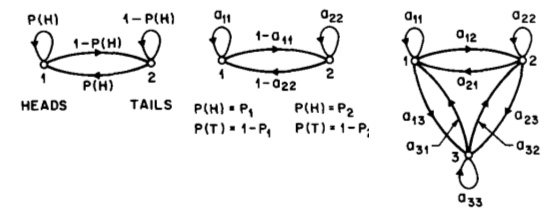
\includegraphics[width=0.85\textwidth]{coin.png}
\end{frame}
\fi




\begin{frame}{HMM: пример}
\begin{block}{Пример: wikipedia}
Доктор опрашивает потенциально больных людей о своем самочувствии и фиксирует ответы. 
Люди могут ответить, что они чувствуют себя нормально (normal), что у них кружится голова (dizzy), что у них озноб (cold).

Наблюдаемые величины $\{O_1, O_2, O_3\} = \{\text{normal, dizzy, cold}\}.$

Скрытые величины --- наличие простуды $\{H_1, H_2\} = \{\text{healthy, fever}\}.$  


\end{block}
\centering
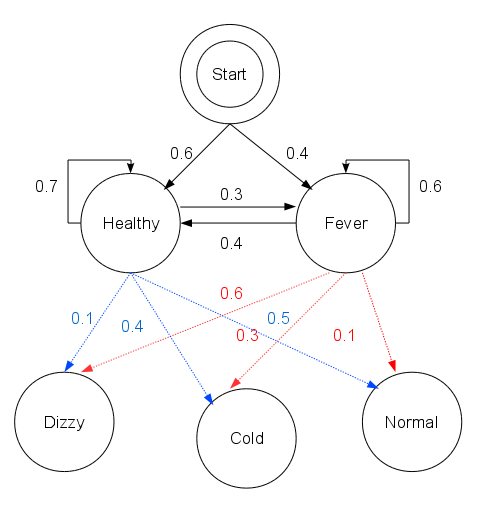
\includegraphics[width=0.25\textwidth]{cold.png}
\end{frame}



\begin{frame}{HMM: основные задачи}
\only<1>
{
\begin{enumerate}
\item Как посчитать вероятность последовательности $X_1, \dots, X_T$?
\item Как выбрать наиболее подходящую скрытую последовательность $H_1,\dots, H_T$ по последовательности $X_1, \dots, X_T$?
\item Как настроить параметры HMM-модели по входной последовательности $X_1, \dots, X_T$?
\end{enumerate}
}
\only<2>
{
\begin{enumerate}
\item Как посчитать вероятность последовательности $X_1, \dots, X_T$?
\item Как выбрать наиболее подходящую скрытую последовательность $H_1,\dots, H_T$ по последовательности $X_1, \dots, X_T$?
\item Как настроить параметры HMM-модели по входной последовательности $X_1, \dots, X_T$?
\end{enumerate}
\textbf{Что интересует нас:}
\begin{enumerate}
\item Как определить адекватность модели?
\item Как выбрать наилучшую модель?
\end{enumerate}
}

\end{frame}
\iffalse

\begin{frame}{HMM: вероятность последовательности}
\textbf{Наивное решение:}  вычисление полной вероятности с полным перебор скрытых состояний:
\[
    P(X_1,\dots,X_N) = \sum_{i_1=1}^n\dots\sum_{i_T=1}^n\pi_{i_1}b_{i_1}(X_1)a_{i_1 i_2}b_{i_2}(X_2)\dots a_{i_{T-1} i_T} b_{i_T}(X_T).
\]
Сложность: $2T\cdot n^T$.

\textbf{Forward-Backward алгоритм.} (будем использовать только Forward-часть)\\
\[
    \alpha_t(i) = P(X_1,\dots,X_t, H_t = S_i).
\] 
Вычисляется по индукции:
\[
\alpha_1(i) = \pi_i b_i(X_1), \quad \alpha_{t+1}(j) = \bigl(\sum_{i=1}^n \alpha_t(i)a_{ij}\bigr)b_j(X_{t+1}).
\]
Итог:
\[
  P(X_1,\dots,X_T) = \sum_{i=1}^n \alpha_T(i).  
\]
Сложность: $O(n^2T)$.
\end{frame}


\begin{frame}{HMM: оптимальная последовательность скрытых состояний}
\textbf{Что такое оптимальная последовательность?}\\
Наивный ответ: будем максимизировать вероятность каждого скрытого состояния по отдельности:
\[
    S_i  = \arg\max_{i'} P(H_t = S_{i'}|X_1,\dots,X_T), \forall t.
\]
\textbf{Проблема:} не учитываются вероятности перехода между скрытыми состояниями $a_{ij}$.

\textbf{Алгоритм Витерби:}
аналогичен Forward-Backward алгоритму:
\[
    \delta_t(i) = \max_{j_1,\dots,j_{t-1}} P(S_{j_1}, \dots,S_{j_{t-1}},S_i, X_1,\dots,X_{t}).
\]
Рекурсивная формула:
\[
    \delta_t(j) = \max_{i} \bigl(\delta_t(i)a_{ij}\bigr)b_j(X_{t+1}).
\]
Для восстановления оптимальной последовательности также требуется завести вспомогательный массив оптимальных состояний $S_t$.
\end{frame}



\begin{frame}{HMM: оптимизация параметров}
\textbf{Алгоритм Баума-Велша}
Алгоритм является EM-алгоритмом.\\
На шаге E:
\[
    \alpha_t(i) = P(X_1,\dots,X_t, H_t = S_i), ~\beta_t(i) =  P(X_{t+1},\dots,X_{T}|H_t = S_i).
\] 
\[
    \xi_t(i,j) = P(H_t= S_i, H_{t+1} = S_{i+1}| X_1,\dots,X_T) = \frac{\alpha_t(i)a_{ij}b_j(X_{t+1})\beta_{t+1}(j)}{\sum_{i',j'}\alpha_t(i')a_{i'j'}b_j(X_{t+1})\beta_{t+1}(j')}.
\]
\[
    \gamma_t(i) = \frac{\alpha_t(i)\beta_t(i)}{\sum_{i'} \alpha_t(i')\beta_t(i')}.
\]
На шаге M:
\begin{itemize}
\item $\pi_i = \gamma_1(i)$ ---  Ожидаемая частота появления $S_i$ на шаге 1.
\item $a_{ij} = \frac{\text{Ожидаемая частота перехода }S_i \to S_j}{\text{Ожидаемая частота появления события } S_i} = \frac{\sum_{t=1}^{T-1}\xi_t(i,j)}{\sum_{t=1}^{T-1}\gamma_t(i)}.$
\item $b_{j}(k) = \frac{\text{Ожидаемая частота появления }S_i \text{ при } O_k}{\text{Ожидаемая частота появления }S_i} = \frac{\sum_{t=1}^{T}\gamma_t(j|O_k)}{\sum_{t=1}^{T}\gamma_t(j)}.$

\end{itemize}
\end{frame}

\fi
\begin{frame}{HMM, основные задачи, наивное решение}

\textbf{Вычисление вероятности последовательности}

Вычисление полной вероятности с полным перебор скрытых состояний:
\[
    P(X_1,\dots,X_N) = \sum_{i_1=1}^n\dots\sum_{i_T=1}^n\pi_{i_1}b_{i_1}(X_1)a_{i_1 i_2}b_{i_2}(X_2)\dots a_{i_{T-1} i_T} b_{i_T}(X_T).
\]
\textbf{Проблема:} высокая сложность: $O(T\cdot n^T)$.

\vspace{1cm}
\textbf{Вычисление оптимальной последовательности скрытых состояний}

Будем максимизировать вероятность каждого скрытого состояния по отдельности:
\[
    S_i  = \arg\max_{i'} P(H_t = S_{i'}|X_1,\dots,X_T), \forall t.
\]
\textbf{Проблема:} не учитываются вероятности перехода между скрытыми состояниями $a_{ij}$.

\end{frame}

\begin{frame}{HMM, основные задачи}
Общепринятые решения основных задач:
\begin{itemize}
\item Вычисление вероятности последовательности: Forward-Backward алгоритм
\begin{itemize}
\item Основан на динамическом программировании
\item Сложность: $O(n^2T)$
\end{itemize}

\item Вычисление оптимальной последовательности скрытых состояний: алгоритм Витерби
\begin{itemize}
\item Основан на динамическом программировании, схож с Forward-Backward алгоритмом
\end{itemize}

\item Оптимизация параметров HMM-модели
\begin{itemize}
\item EM-алгоритм Баума — Велша
\end{itemize}

Подробнее см. Rabiner (в списке литературы).
\end{itemize}

\end{frame}


\begin{frame}{HMM, проверка гипотезы}
\begin{center}
\begin{tabular}{rl}
            выборка:                        & $X_1, \dots, X_T$ \\
            нулевая гипотеза:               & $H_0\colon \mathbf{a} = \mathbf{a}^0, \mathbf{b} = \mathbf{b}^0, \boldsymbol{\pi} = \boldsymbol{\pi}^0.$ \\
            альтернатива:                   & $H_1\colon H_0$ неверна.  \\
            статистика:                     & $2\text{log}\bigl(\hat{p}(X_1,\dots,X_T) - {p}^0(X_1,\dots,X_T)\bigr).$ \\
            нулевое распределение:          & $\chi^2_{n+mn+m^2}$\\
		\end{tabular}
		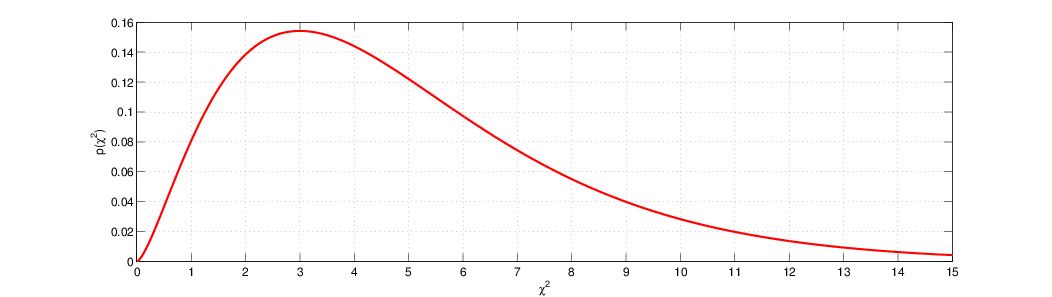
\includegraphics[width=0.85\textwidth]{chi2.png}   
    \end{center}
\end{frame}

\begin{frame}{HMM: сравнение моделей}
\textbf{Как определить понятие эквивалентности на моделях?}\\
Дивергенция Кульбака-Лейблера:
\[
    D_{KL}(p_1,p_2) = \mathsf{E}_{{X} \sim p_2} \bigl(\text{log}p_1({X}) -\text{log}p_2({X})\bigr).
\]
\begin{itemize}
\item $D_{KL}(p_1,p_2)>0.$
\item $D_{KL}(p_1,p_2) \neq D_{KL}(p_2,p_1).$
\item $D_{KL}(p_1,p_2) = 0 <=> p_1 = p_2$.
\end{itemize}

Модификация для HMM:
\[
    D'_{KL}(p_1,p_2) = \frac{1}{N}\mathsf{E}_{{X}_1,\dots,{X}_T \sim p_2} \bigl(\text{log}p_1({X}_1,\dots,{X}_T) -\text{log}p_2({X}_1,\dots,{X}_T)\bigr).
\]

Симметричная версия:
\[
    D''_{KL}(p_1,p_2)  = \frac{    D'_{KL}(p_1,p_2)+     D'_{KL}(p_2,p_1)}{2}. 
\]


\end{frame}

\begin{frame}{HMM: разновидности}
\begin{itemize}
\item left-right-модели
\begin{itemize}
\item Вводится порядок на множестве скрытых наблюдений
\item Переход между наблюдениями ``от большего к меньшему'' запрещен
\item Используется в распознавании речи
\end{itemize}

\item С непрерывным распределением на наблюдениях

\item Авторегрессионные HMM-модели.
%\item С явным указанием продолжительности событий.
\end{itemize}
\end{frame}


\begin{frame}{HMM: эксперимент Cave and Neuwirth}
HMM обучена на большом наборе английских текстов. 
Размерность множества скрытых состояний --- 2. 

Наблюдаемые величины --- символы в тексте.
На выходе получается распределение переходов, при котором скрытую переменную можно интерпретировать как гласную или согласную букву.

\begin{figure}
\centering
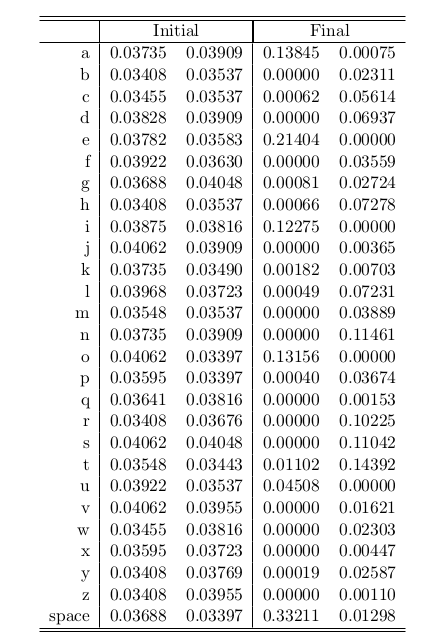
\includegraphics[width=0.25\textwidth]{brown.png}
\end{figure}
\end{frame}

\iffalse

\begin{frame}{IBM Model 1}
%http://mt-class.org/jhu/slides/lecture-ibm-model1.pdf
Решается задача выравнивания предложений на двух языках (e --- English, f --- foreign).
\[
    p(e_1, \dots, e_{l_e}|f_1, \dots, f_{l_f}) = \frac{\epsilon}{(l_f+1)^l_e} \prod_{j=1}^{l_e} p(e_j|f_{a(j)}),
\]
$a$ ---  отображение из позиций ``английских'' слов в иностранные.
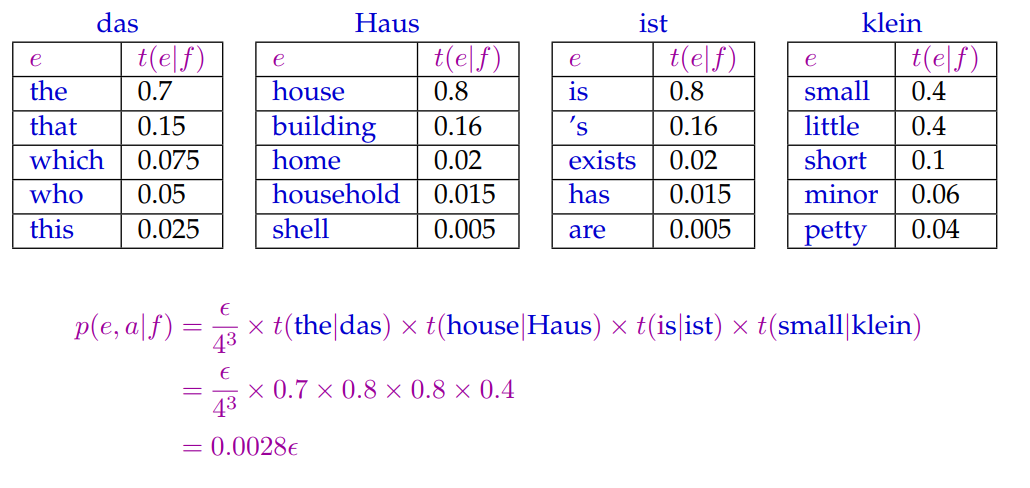
\includegraphics[width=0.85\textwidth]{koehn.png}
\footnotesize
\quad http://mt-class.org/jhu/slides/lecture-ibm-model1.pdf
\end{frame}



\begin{frame}{Машинный перевод: HMM}
\textbf{IBM Model 1:} все выравнивания равнозначны.\\
~\\
\textbf{HMM model:} 
\begin{itemize}
\item Множество скрытых состояний $S_1,\dots,S_n$: множество слов в исходном языке.
\item Множество наблюдений: $O_1,\dots,O_m$: множество слов в языке перевода.
\item Оптимизация параметров: алгоритм Баума-Вэлша.
\item Перевод: Витерби.
\end{itemize}
\end{frame}

\fi 

\begin{frame}{HMM: примеры применения}
\begin{itemize}
\item Назначение соответствий между словами в исходном и переведенном предложении (наблюдения --- множество слов в переведенном предложении, скрытые состояния --- исходные слова). 
\item Анализ частей речи (наблюдения --- слова, скрытые состояния --- части речи).
\item Распознавание речи (наблюдения --- представления звуковых сегментов, скрытые состояния --- слова или буквы).
\item Выравнивание биологических последовательностей (наблюдения --- элементы последовательности, скрытые состояния --- экзоны).
\end{itemize}
\end{frame}

\begin{frame}{Сэмплирующие методы}


\begin{block}{Типовая задача}
Моделируется распределение ходов в стратегическоий игре.

Программист хочет просчитать несколько наиболее типичных ходов компьютера-противника.

Программист также хочет выяснить сколько в среднем юнитов будет у компбютера через несколько ходов.
\end{block}

Марковские модели являются генеративными моделями. Они позволяют ``сэмплировать'' (порождать) объекты из распределения, описываемого марковской моделью.

\textbf{Что делать с более сложными распределениями?}
\begin{itemize}
\item Как сэмплировать?
\item Как вычислять интегралы по этим распределениям?
\end{itemize}

\end{frame}

\begin{frame}{Простые случаи}
\textbf{Интегрирование}

Метод Монте-Карло: проклятье размерности: нужно уметь сэмплировать из нашего распределения

\textbf{Сэмплирование}

Пусть существует обратимая функция $T$ из $x \in \mathcal{U}(0,1)$ в некоторое распределение $z$.
Тогда \[
F_z(t) = p(z \leq t) = p(T(t') \leq t) = p(t' \leq T^{-1}(t)) = T^{-1}(t).
\]
Отсюда $F_z^{-1} = T$.

\textbf{Пример}
\[
    z = \lambda \text{exp}(-\lambda t).
\]
\[
F_z(t) = 1 - \text{exp}(-\lambda t).
\]
\[
F_z^{-1}(t') = -1\frac{1}{\lambda}\text{log}(1-t').
\] 


\end{frame}



\begin{frame}{Сэмплирование с отклонением}
\begin{itemize}
\item Задана плотность $p(z)$ (может быть задана с точностью до нормировочной константы)
\item Введем распределение $q$
\item Подберем множитель $k$ таким образом, чтобы $kq(z) \geq p(z)$ для всех $z$
\item В цикле
\begin{itemize}
\item Просэмплируем $z_0 \sim kq$
\item Просэмплируем $u \sim \mathcal{U}(0, z_0)$
\item Если $u \leq p(z_0)$ --- считать его сэмплом из $p(z)$
\end{itemize}

Идея метода: сэмплы $u$ равномерно распределены в регионе, ограниченном кривой $p(z)$.
\begin{figure}
\centering
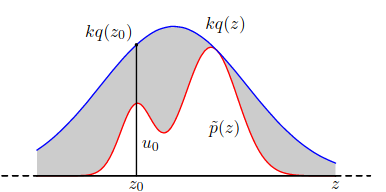
\includegraphics[width=0.3\textwidth]{bishop1.png}
\\Bishop, 2006
\end{figure}

\end{itemize}
\end{frame}


\begin{frame}{Сэмлирование по значимости}
Пусть мы не можем сэмплировать из $p(z)$, но можем оценивать правдоподобие в каждой точке, и хотим получить интерал 
\[
    \mathsf{E}f = \int f(z)p(z)dz.   
\]
Тогда введем распределение $q$:
\[
    \mathsf{E}f = \int f(z)p(z)dz = \int f(z) \frac{p(z)}{q(z)}dz \approx \frac{1}{L} \sum_{l=1}^L \frac{p(z^l)}{q(z^l)}f(z^l).   
\]
\end{frame}

\begin{frame}{MCMC}
\textbf{Основная идея:}
Сэмплируем аналогично сэмплированию с отклонениями, но q --- марковское распределение, обусловленное на предлыдущий успешный шаг

Хотим, чтобы предельное (стационарное) распределение соответствовало нашему распределению $p(z)$.

Достаточное условие
\[
    p(z)T(z|z') = p(z)T(z'|z).
\]
\end{frame}

\begin{frame}{Алгоритм Метрополиса — Гастингса}
\begin{itemize}
\item Сэмплируем новое значение $z' \sim q(z|z^t)$.
\item Принимаем его с вероятностью $A(z'| z^t) = \min\left(1, \frac{p(z')q(z^t|z')}{p(z^t)q(z'|z^t)}\right)$.
\item Если приняли: $z^{t+1} = z'$,
\item иначе: $z^{t+1} = z^t$.
\end{itemize}

Условие предельного распределения выполняется:
\[
    p(z)T(z|z') = p(z)T(z'|z) = p(z')T(z'|z^t) = p(z')q(z'|z^t)A(z'|z^t) = p(z^t)q(z^t|z')A(z^t|z').
\]

\begin{itemize}
\item Сэмплы скоррелированы. Если требуется декоррелировать сэмплы, можно брать каждый $k$-й сэмпл.
\item Работает в пространствах высокой размерности значительно лучше, чем сэмплирование с отклонением.
\end{itemize}
\end{frame}


\begin{frame}{Пример работы,  Andrieu et al.}
\begin{figure}
\centering
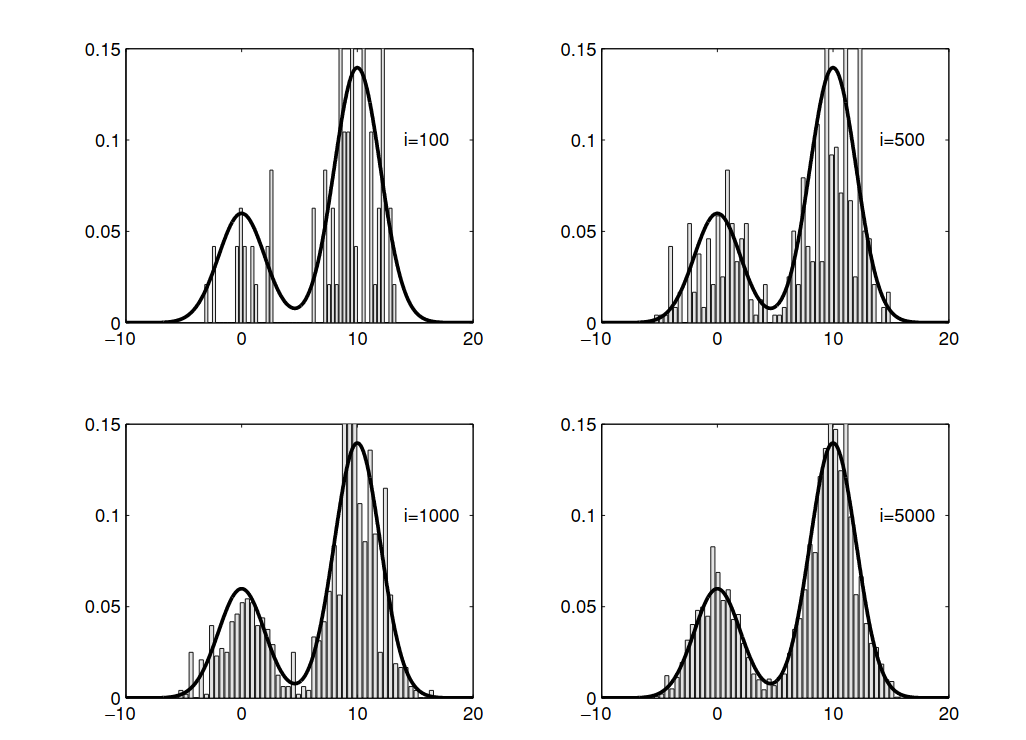
\includegraphics[width=0.5\textwidth]{and.png}
\end{figure}
\end{frame}


\begin{frame}{Литература}
\begin{itemize}
\item Tutorial: L. R. Rabiner, A Tutorial on Hidden Markov Models and Selected Applications in Speech Recognition
\item Tutorial: M. Stamp, A Revealing Introduction to Hidden Markov Models
\item Проверка гипотез: T. W. Anderson, Leo A. Goodman, Statistical Inference about Markov Chains
\item Языковые модели: D. Jurafsky, J. H. Martin, Speech and Language Processing
\item Машинный перевод:  P. Koehn, Statistical Machine Translation
\item IBM M1 \& HMM: http://www.cs-114.org/wp-content/uploads/2016/04/CS114\_L25PMachineTranslation-IBM.pdf
\item Bishop C. M. Pattern recognition and machine learning. – springer, 2006.
\item Andrieu C. et al. An introduction to MCMC for machine learning //Machine learning. – 2003. – Т. 50. – №. 1. – С. 5-43.
\end{itemize}
\end{frame}

\end{document}
